\section{The Safety Annex}
\label{sec:safety_annex}

In this section, we describe the main features and functionality of the Safety Annex. The usage of the terms error, failure, and fault follow their definitions in Section~\ref{sec:terminology}. We use {\em fault} as the generic modeling keyword throughout the AADL model hierarchy.

The Safety Annex Users Guide can be found at \url{https://github.com/loonwerks/AMASE/tree/develop} along with the tool plugins and examples described in this report. 

\subsection{Modeling Language for System Design}
\label{subsec:aadl}
We are using the Architectural Analysis and Design Language (AADL) to construct system architecture models~\cite{FeilerModelBasedEngineering2012}.  AADL is an SAE International standard that defines a language and provides a unifying framework for describing the system architecture for ``performance-critical, embedded, real-time systems''~\cite{AADL_Standard}. From its conception, AADL has been designed for the design and construction of avionics systems.  Rather than being merely descriptive, AADL models can be made specific enough to support system-level code generation.  Thus, results from analyses conducted, including the new safety analysis proposed here, correspond to the system that will be built from the model.  

An AADL model describes a system in terms of a hierarchy of components and their interconnections, where each component can either represent a logical entity (e.g., application software functions, data) or a physical entity (e.g., buses, processors). An AADL model can be extended with language annexes to provide a richer set of modeling elements for various system design and analysis needs (e.g., performance-related characteristics, configuration settings, dynamic behaviors). The language definition is sufficiently rigorous to support formal analysis tools that allow for early phase error/fault detection.






\subsection{Modeling Language for System Design}
\label{subsec:aadl-agree}
We are using the Architectural Analysis and Design Language (AADL)~\cite{FeilerModelBasedEngineering2012} to construct system architecture models.  AADL is an SAE International standard that defines a language and provides a unifying framework for describing the system architecture for ``performance-critical, embedded, real-time systems''~\cite{AADL_Standard}. From its conception, AADL has been designed for the design and construction of avionics systems.  
Rather than being merely descriptive, AADL models can be made specific enough to support system-level code generation.  Thus, results from analyses conducted, including the new safety analysis proposed here, correspond to the system that will be built from the model.  

An AADL model describes a system in terms of a hierarchy of components and their interconnections, where each component can either represent a logical entity (e.g., application software functions, data) or a physical entity (e.g., buses, processors). An AADL model can be extended with language annexes to provide a richer set of modeling elements for various system design and analysis needs (e.g., performance-related characteristics, configuration settings, dynamic behaviors). The language definition is sufficiently rigorous to support formal analysis tools that allow for early phase error/fault detection.

The Assume Guarantee Reasoning Environment (AGREE)~\cite{NFM2012:CoGaMiWhLaLu} is a tool for formal analysis of behaviors in AADL models.  It is implemented as an AADL annex and annotates AADL components with formal behavioral contracts. Each component's contracts can include assumptions and guarantees about the component's inputs and outputs respectively, as well as predicates describing how the state of the component evolves over time. AGREE translates an AADL model and the behavioral contracts into Lustre~\cite{Halbwachs91:IEEE} and then queries a user-selected
model checker to conduct the back-end analysis. The analysis %is
can be performed compositionally following the architecture hierarchy such that analysis at a higher level is based on the components at the next lower level.  When compared to monolithic analysis (i.e., analysis of the flattened model composed of all components), the compositional approach allows the analysis to scale to much larger systems~\cite{NFM2012:CoGaMiWhLaLu}. 

%In the avionics context, the software functions/applications, the hardware equipment, and the system that is composed of their integration can all be represented as components connected to/composed of/bind to other components in a hierarchical AADL model. AGREE contracts can be used to capture the functional requirements at each level of the hierarchy. Once the model has been reviewed and the requirements captured have been validated, the back-end analysis can be conducted to verify if each level of the model implements its higher level requirements correctly.

%AADL with the AGREE extension serves as a good candidate as the modeling language for describing the system design aspects of a shared system design and safety analysis model. 
In our prior work~\cite{Stewart17:IMBSA}, we added an initial failure effect modeling capability to the AADL/AGREE language and tool set.  We are continuing this work so that our tools and methodology can be used to satisfy system safety objectives of ARP4754A and ARP4761.  

\begin{comment}
In particular, our goals are to:

\begin{itemize}
	\item Provide a comprehensive, qualitative description of the causal relationship between basic failure events and system level safety requirements.
	\item Provide an accurate, quantitative description of the contribution relationship between failure rates of the fault tree basic events and numerical probability requirements at the system level.
\end{itemize}
\end{comment}
%The remainder of the paper describes our approach towards both of the goals.





\subsection{Basic Functionality of the Safety Annex}

An AADL model of the nominal system behavior specifies the hardware and software components of the system and their interconnections. This nominal model is then annotated with assume-guarantee contracts using the AGREE annex for AADL. The nominal model requirements are verified using compositional verification techniques based on inductive model checking~\cite{2017arXiv171201222G}.

Once the nominal model behavior is defined and verified, the Safety Annex can be used to specify possible faulty behaviors for each component. The faults are defined on each of the relevant components using a customizable library of fault nodes and the faults are assigned a probability of occurrence. A probability threshold is also defined at the system level. This extended model can be analyzed to verify the behavior of the system in the presence of faults. Verification of the nominal model with or without the fault model is controlled through the safety analysis option during AGREE verification.

To illustrate the syntax of the Safety Annex, we use an example based on the Wheel Brake System (WBS) described in AIR6110 standards document and used in  previous work ~\cite{Stewart17:IMBSA, AIR6110}.

The \textit{fault library} contains commonly used fault node definitions. Commonly used faults in various systems include \textit{fail\_to} fault, where the output of a component fails to a particular value, for instance a pump may fail to produce any output and hence the fail to value is zero. Another example of a commonly occuring fault is an \textit{inverted\_boolean}. For example, a sensor may have an inverted value fault present on its boolean output. The fault library is simply a collection of fault nodes with these commonly used fault definitions which are then easily referenced within the fault definitions in the safety annex. 


A \textit{fault declaration} is shown in Figure~\ref{fig:fault_pump}. This describes a fail to zero fault in a pump. The \textit{fail\_to} node provides the mechanism in which a faulty value is injected into the fault model. When the \textit{trigger} condition for this pump fault is satisfied, the nominal component output value is overridden by the failure value. In this particular example, the pump will fail to produce any pressure and the hydraulic fluid ceases being pumped through the lines.  

\begin{figure*}[h!]
	\vspace{-0.6in}
	\begin{center}
		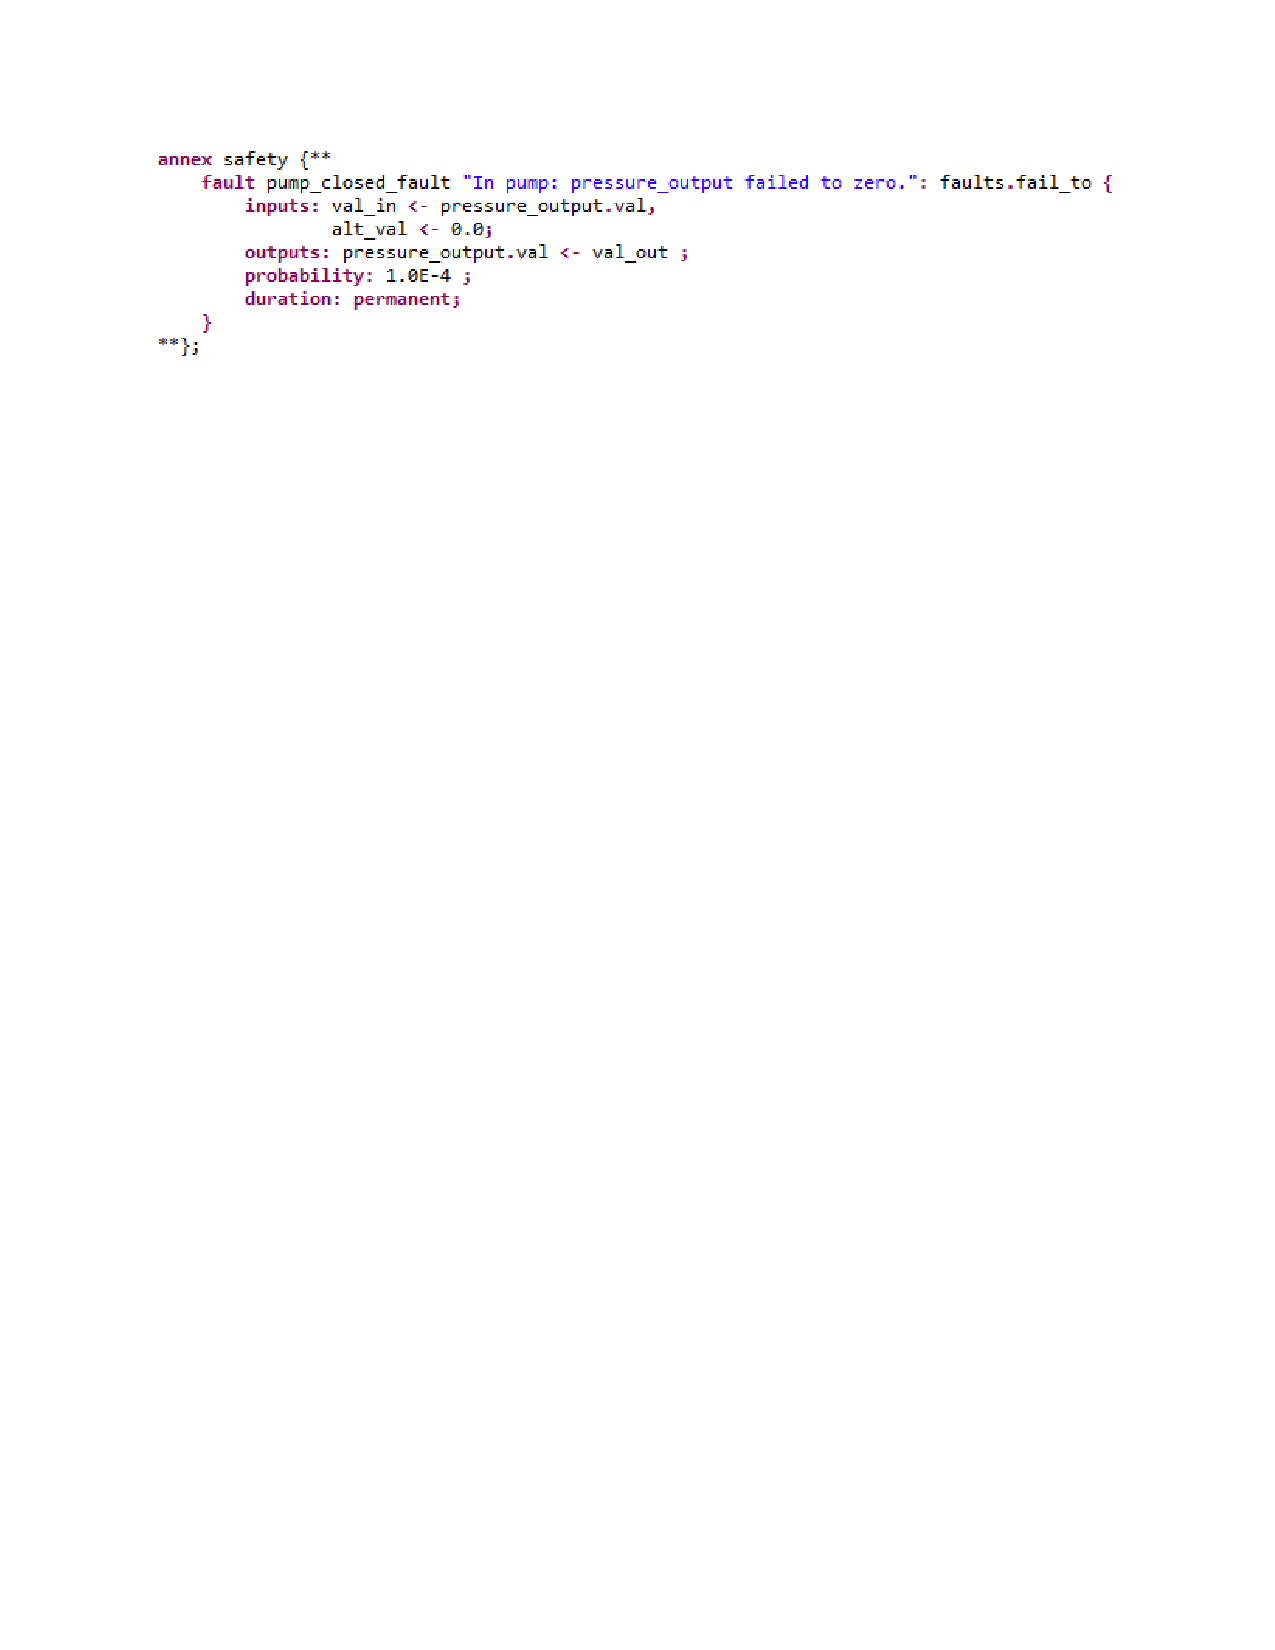
\includegraphics[trim=30 635 0 30,clip,width=1.3\dimexpr\textwidth-1.5cm\relax]{images/pump_fault.pdf}
		\caption{Pump Fault Definition in the Safety Annex}
		\label{fig:fault_pump}
	\end{center}
\end{figure*}

The \textit{fault statement} consists of a unique description string, the fault node definition name, and a series of \textit{fault subcomponent} statements. Contents of the fault statement are as follows.\\
\textbf{Inputs} in a fault statement are the parameters of the fault node definition. In the example above, \textit{val\_in} and \textit{alt\_val} are the two input parameters of the fault node. These are linked to the output from the Pump component (\textit{pressure\_output.val}), and \textit{alt\_value}, a fail to value of zero. When the analysis is run, these values are passed into the fault node definition.\\
\textbf{Outputs} of the fault definition correspond to the outputs of the fault node. The fault output statement links the component output (\textit{pressure\_output.val}) with the fault node output (\textit{val\_out}). If the fault is triggered, the nominal value of \textit{pressure\_output.val} is overridden by the failure value output by the fault node. Faulty outputs can take deterministic or non-deterministic values. \\
\textbf{Probability} (optional) describes the probability of a fault occurrence.\\
\textbf{Duration} describes the duration of the fault; currently the Safety Annex supports permanent faults.\\

\subsection{Hardware Failures and Dependent Faults}

Failures in hardware (HW) components can trigger behavioral faults in the software (SW) or system (SYS) components that depend on them.  For example, a CPU failure may trigger faulty behavior in threads bound to that CPU. In addition, a failure in one HW component may trigger failures in other HW components located nearby, such as cascading failure caused by a fire or water damage.

Faults propagate in AGREE as part of the nominal behavior of a system. This means that any propagation in the HW portion of an AADL model would have to be artificially modeled using data ports and AGREE behaviors in SW. This is less than ideal as there may not be concrete behaviors associated with HW components. In other words, faulty behaviors mainly manifest themselves on the software components that depend on the hardware components.

To better model faults at the system level dependent on HW failures, there is a fault definition specifically designed for HW components. In comparison to the basic fault statement introduced in the previous section, users are not specifying behavioral effects for the HW failures, nor data ports to apply the failure. An example of a hardware component fault declaration is shown in Figure~\ref{fig:hardware_fault}.

\begin{figure}[h!]
	\begin{center}
		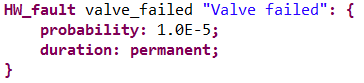
\includegraphics[width=.4\textwidth]{images/hw_fault.png}
		\caption{Hardware Fault in the Safety Annex}
		\label{fig:hardware_fault}
	\end{center}
\end{figure}

%\noindent
%\begin{minipage}{\textwidth}% to keep image and caption on one page
%\makebox[\linewidth]{%        to center the image
%  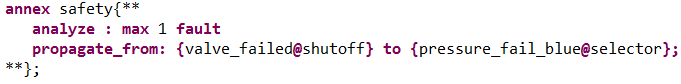
\includegraphics[keepaspectratio=true,scale=0.6]{images/fault_propagation.png}}
%\captionof{figure}{Fault Propagation}
%\label{fig:fault_propagation}%      only if needed  
%\end{minipage}

\begin{figure*}[]
	\begin{center}
		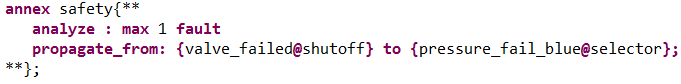
\includegraphics[width=.7\textwidth]{images/fault_propagation.png}
		\caption{Fault Propagation}
		\label{fig:fault_propagation}
	\end{center}
\end{figure*}

When analyzing hardware specific faults, it is often of interest to see how these faults may propagate to other components of the system, specifically the software components. As an example, consider software systems that run on a particular CPU. This CPU has a hardware fault pertaining to overheating. An important question is how this hardware specific fault may propagate to components that rely on the CPU. In the nominal model, there is a binding between hardware and software components in AADL that is specified within the system implementation. In order to model this type of fault, users can specify fault dependencies in the system implementation where these dependencies are clearly defined. This is the only case of explicit fault propagation within the Safety Annex and in this case the propagation only is from the hardware to the software that runs on it. An example of a fault dependency specification is shown in Figure~\ref{fig:fault_propagation}, showing that a valve failure triggers a pressure failure fault at a subcomponent that relies upon that valve. 


\subsection{Implementation Details}

\begin{figure*}[h!]
\begin{center}
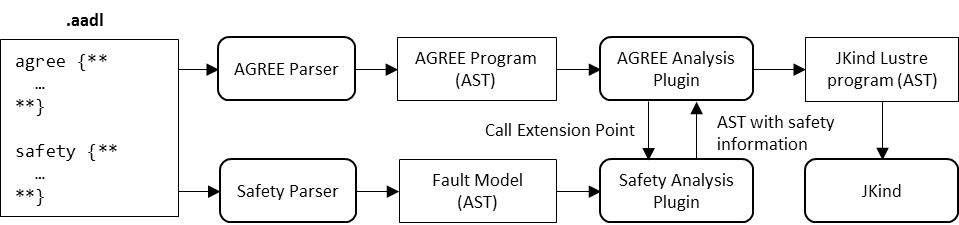
\includegraphics[width=.9\textwidth]{images/arch.png}
\vspace{0.1in}
\caption{Safety Annex Plug-in Design}
\label{fig:plugin-arch}
\end{center}
\end{figure*}

This section provides an overview of how the Safety Annex is related to AADL, AGREE, and the JKind model checker.  The Safety Annex is written in Java as a plug-in for the OSATE AADL toolset, which is built on Eclipse.  It is not designed as a stand-alone extension of the language, but works with behavioral contracts specified AGREE annex and associated tools.  AGREE allows assume-guarantee behavioral contracts to be added to AADL components.  The language used for contract specification is based on the Lustre dataflow language~\cite{Halbwachs91:IEEE}. 

The organization of these interactions  is shown in Figure~\ref{fig:plugin-arch}. The AADL file is annotated with AGREE contracts which creates the nominal model. This nominal model is parsed and sent to JKind where formal verification is performed. If the Safety Annex is also annotated within this model, this creates the extended (fault) model. When desired, the user can run ``Perform Safety Analysis'' within the Osate environment. This creates an extension point where the Safety Analysis informaiton is added into the AGREE model before getting passed to JKind for analysis. In either case, the JKind verification result is returned and displayed to the user in the Osate environment. For more information about this process or figures depicting the environment and analysis results, see the Safety Annex Users Guide or the Safety Annex Technical Report~\cite{amaseRepo, SATechReport}.



%AGREE contracts are used to define the nominal behaviors of system components as {\em guarantees} that hold when {\em assumptions} about the values the component's environment are met.  The Safety Annex extends these contracts to allow faults to modify the behavior of component inputs and outputs.  To support these extensions, AGREE implements an Eclipse extension point interface that allows other plug-ins to modify the generated abstract syntax tree (AST) prior to its submission to the solver.  If the Safety Annex is enabled, these faults are added to the AGREE contract and, when triggered, override the nominal guarantees provided by the component.  An example of a portion of an initial AGREE node and its extended contract is shown in Figure~\ref{fig:comp}.  The \texttt{\_\_fault} variables and declarations are added to allow the contract to override the nominal behavioral constraints (provided by guarantees) on outputs.  In the Lustre language, \texttt{assertion}s are constraints that are assumed to hold in the transition system.

%\begin{figure}
%\vspace{-0.1in}
%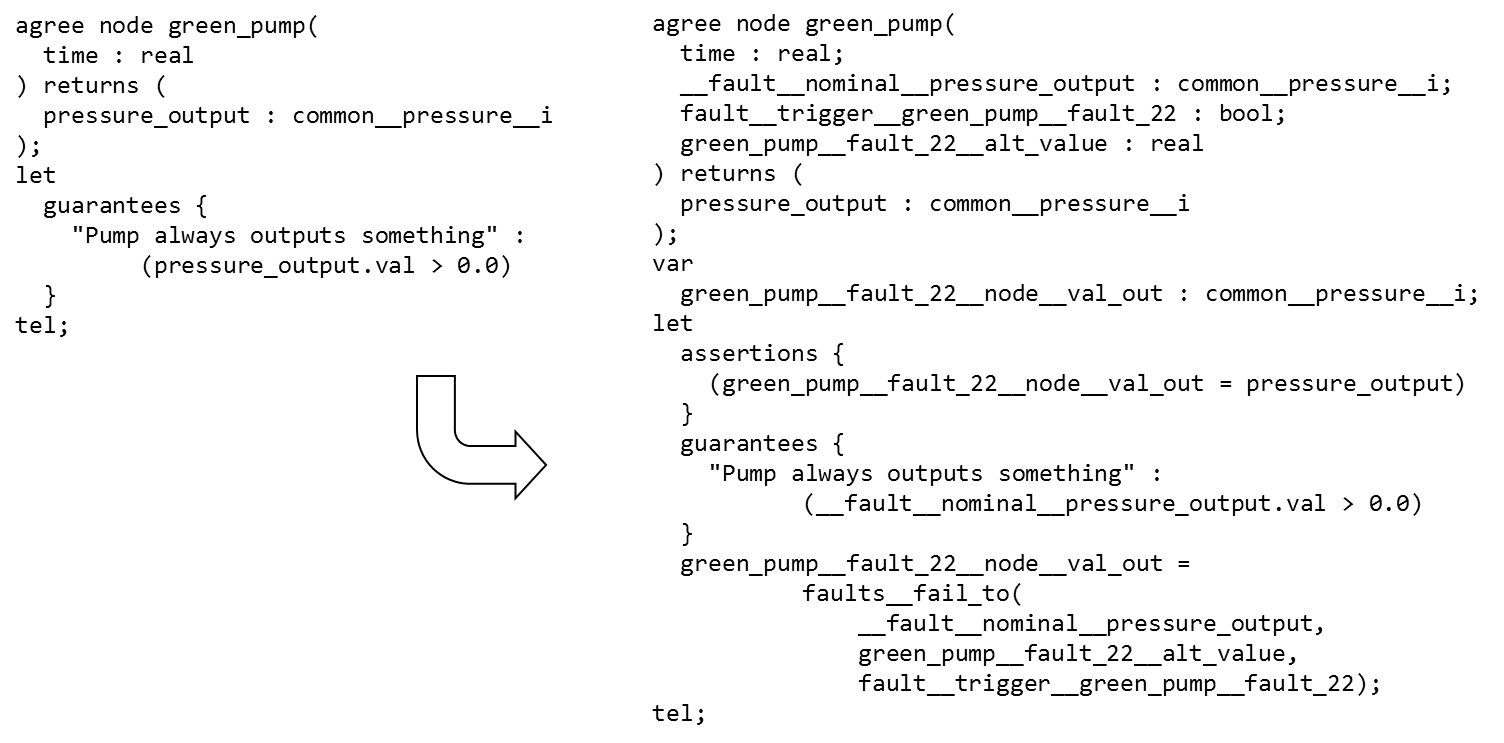
\includegraphics[width=\textwidth]{images/sample_code.png}
%\vspace{-0.3in}
%\caption{Nominal AGREE node and its extension with faults}
%\label{fig:comp}
%\end{figure}

%An annotation in the AADL model determines the fault hypothesis.  This may specify either a maximum number of faults that can be active at any point in execution (typically one or two), or that only faults whose probability of simultaneous occurrence is above some probability threshold should be considered.  In the former case, we assert that the sum of the true {\em fault\_\_trigger} variables is below some integer threshold.  In the latter, we determine all  combinations of faults whose probabilities are above the specified probability threshold, and describe this as a proposition over {\em fault\_\_trigger} variables.

%Once augmented with fault information, the AGREE model follows the standard AGREE translation path to the model checker JKind~\cite{2017arXiv171201222G}, an infinite-state model checker for safety properties.  The augmentation includes traceability information so that when counterexamples are displayed to users, the active faults for each component are visualized.


